\subsubsection{UC10 - Ricerca funzione tramite keyword}
\begin{figure}[H]
	\centering
	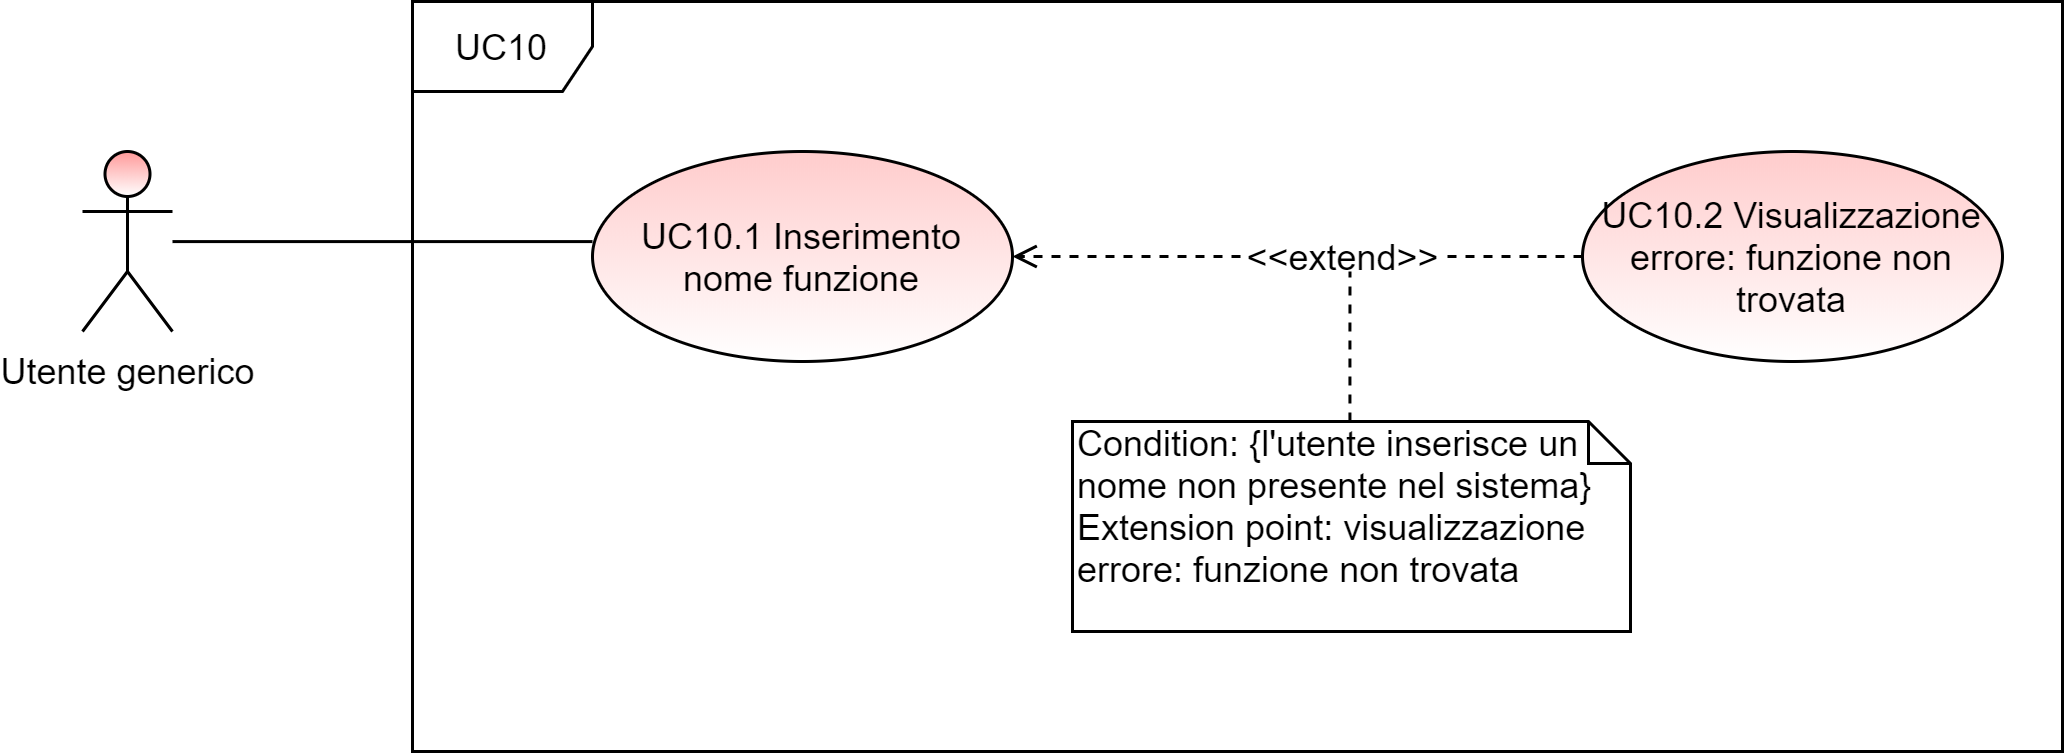
\includegraphics[scale=\ucs]{./res/img/UC10.png}
	\caption {UC10 - Ricerca funzione tramite keyword}
\end{figure}
\begin{itemize}
	\item \textbf{Attori primari:} \ua{};
	\item \textbf{Attori secondari:} \re{};
	\item \textbf{Descrizione:} l’utente richiede di eseguire la ricerca di tutte le funzioni il cui nome contiene una certa keyword eseguendo il comando \psearch{};
	\item \textbf{Scenario principale:} l’utente inserisce correttamente ed esegue il comando \psearch{}; 
	\item \textbf{Precondizione:} l’utente desidera individuare tutte le funzioni correlate ad un certo termine;
	\item \textbf{Postcondizione:} viene eseguita la ricerca di tutte le funzioni il cui nome contiene il termine di ricerca specificato nel comando \search{}.
\end{itemize}